\documentclass{article}
\usepackage[utf8]{inputenc}
\usepackage{geometry}
 \geometry{
 a4paper,
 total={170mm,257mm},
 left=20mm,
 top=20mm,
 }
\usepackage{polski}
\usepackage{natbib}
\usepackage[capbesideposition=right]{floatrow}
\usepackage{graphicx}
\usepackage{pbox}
\usepackage{float}
\usepackage[dvipsnames]{xcolor}
\usepackage{caption}
\usepackage{wrapfig}
\usepackage{graphicx}
\usepackage{tikz}
    \usetikzlibrary{
        arrows,
        shadows,
        shapes,
        automata,
        positioning,
        arrows.meta
    }
\usepackage{pgfplots}
\usepackage{tabularx}
\usepackage{booktabs}
\usepackage{amsfonts}
\pgfplotsset{compat=1.17}

\begin{document}
\centering 
\Huge Sequence diagram of tasks in simulation
\vspace{1cm}
\normalsize
    
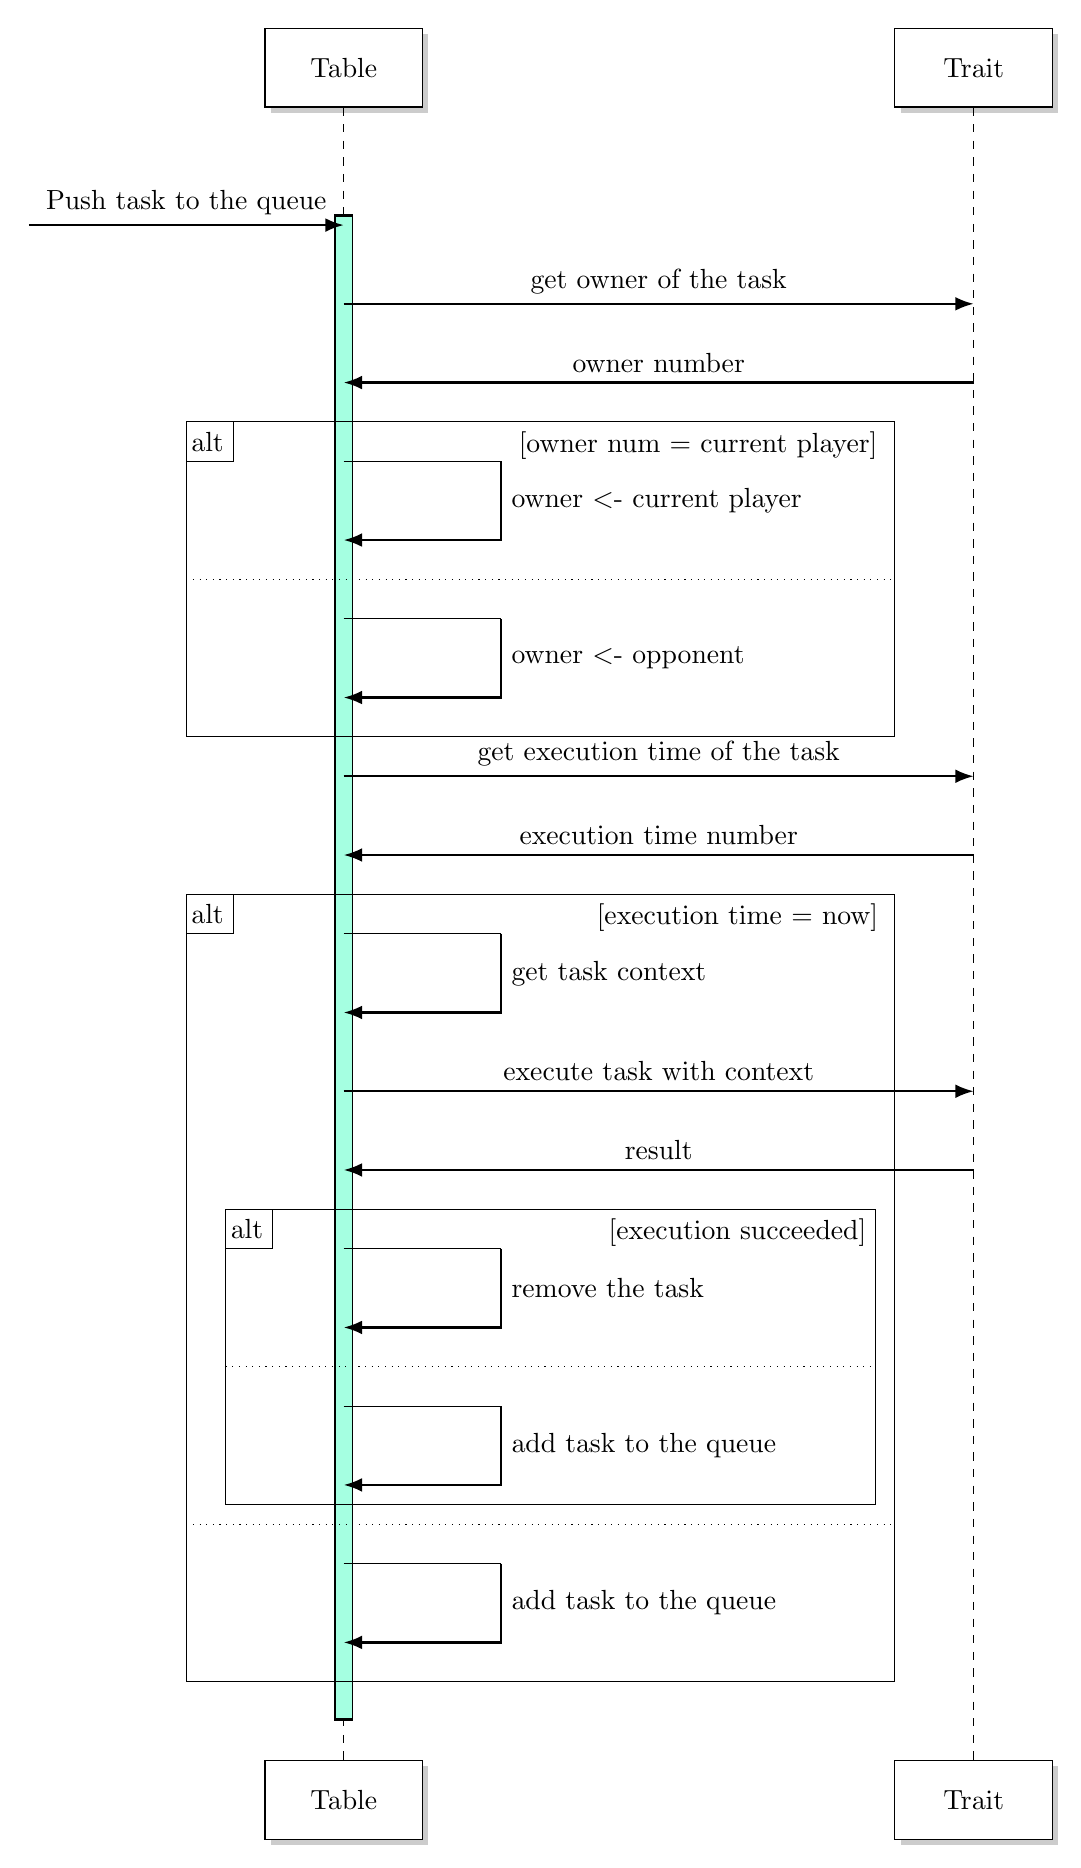
\begin{tikzpicture}
[baseshape/.style={minimum width=2cm, minimum height=1cm,text centered, font=\normalsize,draw=black, drop shadow=black!40},
startstop/.style={baseshape, ellipse, fill=red!30},
io/.style={baseshape, trapezium, trapezium stretches=true, 
trapezium left angle=70, trapezium right angle=110, fill=blue!30},
process/.style={baseshape, rectangle, rounded corners, fill=orange!15},
decision/.style={baseshape, diamond, fill=green!30, text width=1.5cm},
block/.style={baseshape, rectangle, fill=white},
arrow/.style={thick, -Latex},
node distance=2cm,]
\node (step0a) [block] {Table};
\node (step0b) [block, right of =step0a, xshift = 6cm] {Trait};

\node (stopa) [block, below of =step0a, yshift = -20cm] {Table};
\node (stopb) [block, below of =step0b, yshift = -20cm] {Trait};

\draw [dashed] (step0a) -- (stopa);
\draw [line width = 0.24cm] (0, -1.86) -- (0, -21);
\draw [line width = 0.2cm, Aquamarine!70] (0, -1.9) -- (0, -20.96);
\draw [dashed] (step0b) -- (stopb);

\draw[arrow] (-4, -2) -- node[anchor = south]{Push task to the queue}(0,-2);

\draw[arrow] (0, -3) -- node[anchor = south]{get owner of the task}(8, -3);
\draw[arrow] (8, -4) -- node[anchor = south]{owner number}(0, -4);

\draw (-2, -4.5) -| node[at start, xshift = 6.5cm, anchor = north]{$[$owner num = current player$]$}(7, -8.5) -| (-2, -4.5) -| (-1.4, -5) -| node[at start, anchor = south east]{alt}(-2, -4.5);
\draw [dotted] (-2, -6.5) -- (7, -6.5);

\draw (0, -5) -- (2, -5);
\draw[arrow] (2, -5) |- node[near start,anchor = west]{owner $<$- current player}(0, -6);

\draw (0, -7) -- (2, -7);
\draw[arrow] (2, -7) |- node[near start,anchor = west]{owner $<$- opponent}(0, -8);

\draw [arrow] (0, -9) -- node[anchor = south]{get execution time of the task}(8, -9);
\draw [arrow] (8, -10) -- node[anchor = south]{execution time number}(0, -10);

\draw (-2, -10.5) -| node[at start, xshift = 7cm, anchor = north]{$[$execution time = now$]$}(7, -20.5) -| (-2, -10.5) -| (-1.4, -11) -| node[at start, anchor = south east]{alt}(-2, -10.5);
\draw [dotted] (-2, -18.5) -- (7, -18.5);

\draw (0, -11) -- (2, -11);
\draw[arrow] (2, -11) |- node[near start,anchor = west]{get task context}(0, -12);

\draw [arrow] (0, -13) -- node[anchor = south]{execute task with context}(8, -13);
\draw [arrow] (8, -14) -- node[anchor = south]{result}(0, -14);

\draw (-1.5, -14.5) -| node[at start, xshift = 6.5cm, anchor = north]{$[$execution succeeded$]$}(6.75, -18.25) -| (-1.5, -14.5) -| (-0.9, -15) -| node[at start, anchor = south east]{alt}(-1.5, -14.5);
\draw [dotted] (-1.5, -16.5) -- (6.75, -16.5);

\draw (0, -15) -- (2, -15);
\draw[arrow] (2, -15) |- node[near start,anchor = west]{remove the task}(0, -16);

\draw (0, -17) -- (2, -17);
\draw[arrow] (2, -17) |- node[near start,anchor = west]{add task to the queue}(0, -18);

\draw (0, -19) -- (2, -19);
\draw[arrow] (2, -19) |- node[near start,anchor = west]{add task to the queue}(0, -20);













\end{tikzpicture}
\end{document}